\hspace{3em}
Gitlab est un logiciel rendant la manipulation d’un projet utilisant git beaucoup plus simple grâce à une multitude de fonctionnalités. Nous en avons principalement utilisé deux : le gestionnaire de ticket ainsi que les merge request.

	Le gestionnaire de ticket permet d’avoir un suivi des tâches à réaliser, déjà réalisées et en cours de réalisation. Chaque chose à faire pour le projet est traduite en tâche plus ou moins atomique, certaines correspondent à un “ensemble de choses à faire” qui sont assez courtes et ont donc le même objectif. Ainsi il a été possible d’attribuer des issues (nom donné aux tickets) aux membres du groupe pour que chacun ai des choses à faire. Nous avons aussi utilisé une nomenclature pour l’écriture des issues et leur manipulation : sur leur nom, et sur leur état.

	Le nom d’une issue doit prendre la forme :

	TYPE\_ISSUE : Nom issue

Le nom de l’issue doit être assez descriptif pour que l’on comprenne à quoi elle correspond, mais assez courte car il y a un champs description justement fait pour cela.
Le type d’issue n’est pas natif dans gitlab contrairement à d’autres gestionnaires de ticket comme Jira, mais il nous a paru important d’identifier à quoi servent chaque issues.
Les types possibles sont les suivants :

\textbf{BUGFIX} : Le ticket est ouvert car une fonctionnalité présente un bug et il doit être corrigé

\textbf{FONCTIONNALITÉ} : L’issue apporte un contenu fonctionnel à l’utilisateur final (exemple : jouer une partie)

\textbf{TACHE} : L’issue doit être réalisée mais en soit elle ne présente aucun intérêt pour l’utilisateur final car lui ne verra pas le résultat (exemple : écriture de tests)

\textbf{SOUS-TACHE} : Les tâches ont parfois besoin d’être divisées en sous-tâches pour être mieux réparties entre les développeurs. La tâche correspond alors à un ensemble fonctionnel. Une sous-tâche ne peut pas elle même avoir de sous tâche. Le nom d’une issue de type sous-tâche est précédé d’un \# avec le numéro de l’issue à laquelle elle fait référence.

	L’autre utilité de Gitlab a été les merge request. Une merge request est une demande de fusion entre une branche A et une autre branche B. Ce qui veut dire que les branches A et B vont être mélangées commit par commit pour que tous les changements de la branche A soient intégrés dans la branche B.
Grâce à Gitlab les développeurs peuvent alors visionner les changements apportés par la branche A par rapport à la B, donner leur avis, et approuver la demande de merge.
Chaque développeur peut alors voir le travail fourni par les autres lorsqu’ils souhaitent proposer leurs modifications au projet, et apporter un oeil nouveau sur le travail produit. Une fois tous les commentaires validés sur la merge request, elle est prête à être “merge” directement sur la branche master.

\begin{center}
\textbf{Exemple de commentaire sur une merge request}
\end{center}
\begin{figure}[h]
  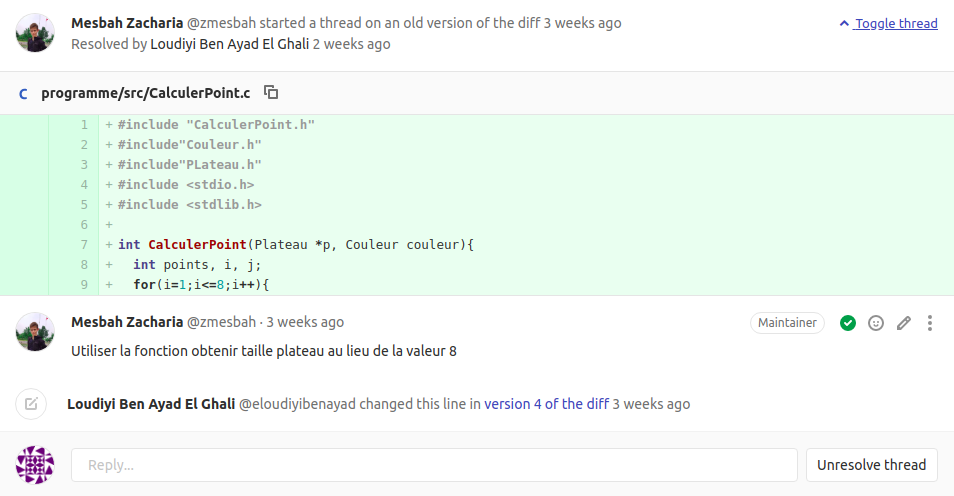
\includegraphics[width=18cm]{./sourcesIMAGES/exempleMergeRequest.png}
  \caption{Ici, Zacharia fait une remarque sur un bout de code produit par El Ghali}
\end{figure}
